\documentclass[6pt]{scrartcl}
\usepackage{tkz-berge}
\begin{document}
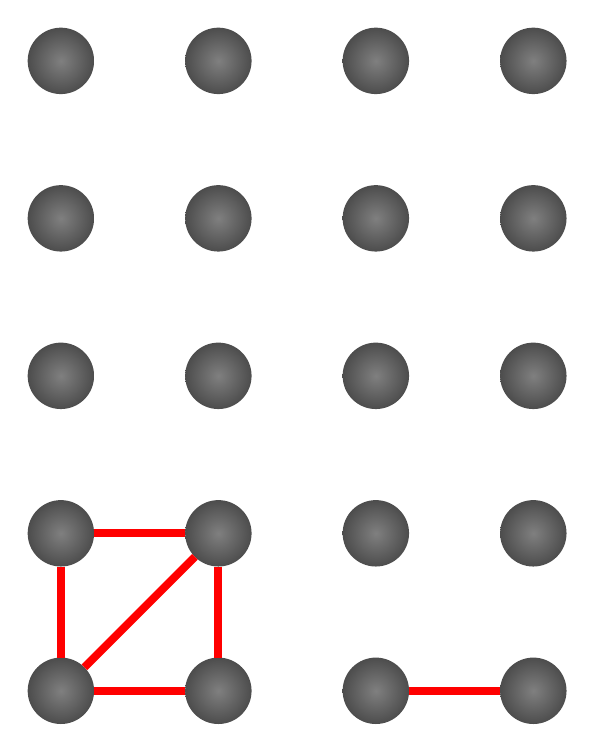
\begin{tikzpicture}[scale=1]
  \SetVertexNoLabel
  %\GraphInit[vstyle=Classic]
  \tikzset{VertexStyle/.style={%ball color=black,fill=black
      shape=circle,outer color=black!70, inner color=black!50, inner sep=8pt,minimum size=24pt},
    EdgeStyle/.style={red,line width=1mm}
  }
  \grEmptyPath[Math,prefix=a,RA=2,RS=0]{4}
  \grEmptyPath[Math,prefix=b,RA=2,RS=2]{4}
  \grEmptyPath[Math,prefix=c,RA=2,RS=4]{4}
  \grEmptyPath[Math,prefix=d,RA=2,RS=6]{4}
  \grEmptyPath[Math,prefix=e,RA=2,RS=8]{4}
  \EdgeInGraphSeq{a}{0}{0}
  \EdgeInGraphSeq{a}{2}{2}
  \EdgeInGraphSeq{b}{0}{0}
  \EdgeIdentity{a}{b}{2}
  \EdgeFromOneToSeq{a}{b}{0}{1}{1}
\end{tikzpicture}
\end{document}